\documentclass[12pt,letterpaper]{hmcpset}
\usepackage[margin=1in]{geometry}
\usepackage{graphicx}

% info for header block in upper right hand corner
\name{ }
\class{Math 60}
\assignment{HW 8}
\duedate{Thursday, May 26, 2016}

\newcommand{\pn}[1]{\left( #1 \right)}
\newcommand{\abs}[1]{\left| #1 \right|}
\newcommand{\bk}[1]{\left[ #1 \right]}

\newcommand{\RR}{\mathbb{R}}

\renewcommand{\labelenumi}{{(\alph{enumi})}}

\begin{document}

\problemlist{5.2.\{7, 14\}, 5.3.\{1, 13, 18\}, 5.4.\{4, 5, 18, 29ab\}}

\begin{problem}[Colley 5.2.7]
    In Exercises 4-13, evaluate the given iterated integrals. In
    addition, sketch the regions $D$ that are determined by the limits
    of integration.
    \[
        \int_{-1}^3\int_x^{2x+1}xy\ dy\ dx
    \]
\end{problem}
\begin{solution}
    \vfill
\end{solution}
\newpage

\begin{problem}[Colley 5.2.14]
    Figure 5.43 shows the level curves indicating the varying depth
    (in feet) of a 25 ft by 50 ft swimming pool. Use a Riemann sum to
    estimate, to the nearest 100 ft$^3$, the volume of water that the
    pool contains.
    \begin{center}
        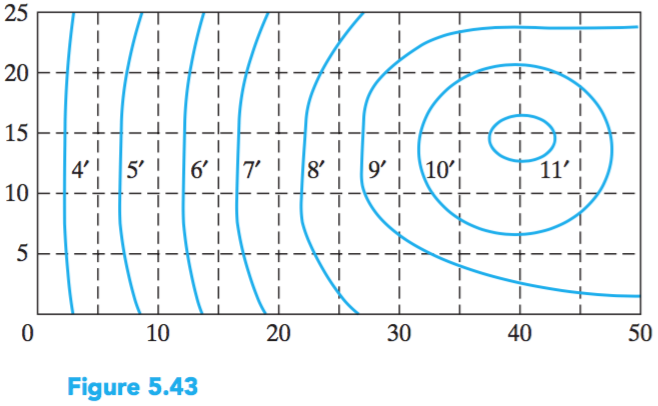
\includegraphics[scale=0.8]{img/5_2_14}
    \end{center}
\end{problem}
\begin{solution}
    \vfill
\end{solution}
\newpage

\begin{problem}[Colley 5.3.1]
    Consider the integral
    \[
        \int_0^2\int_{x^2}^{2x}(2x+1)\ dy\ dx.
    \]
    \begin{enumerate}
        \item Evaluate this integral.
        \item Sketch the region of integration. 
        \item Write an equivalent iterated integral with the order of
            integration reversed. Evaluate this new integral and check
            that your answer agrees with part (a).
    \end{enumerate}
\end{problem}
\begin{solution}
    \vfill
\end{solution}
\newpage

\begin{problem}[Colley 5.3.13]
    In Exercises 12 and 13, rewrite the given sum of iterated
    integrals as a single iterated integral by reversing the order of
    integration, and evaluate.
    \[
        \int_0^8\int_0^{\sqrt{y/3}}y\ dx\ dy+
        \int_8^{12}\int_{\sqrt{y-8}}^{\sqrt{y/3}}y\ dx\ dy
    \]
\end{problem}
\begin{solution}
    \vfill
\end{solution}
\newpage

\begin{problem}[Colley 5.3.18]
    In Exercises 14-18, evaluate the given iterated integral.
    \[
        \int_0^2\int_{y/2}^1e^{-x^2}\ dx\ dy
    \]
\end{problem}
\begin{solution}
    \vfill
\end{solution}
\newpage

\begin{problem}[Colley 5.4.4]
    Find the value of $\iiint_Wz\ dV$, where
    $W=[-1,2]\times[2,5]\times[-3,3]$, without resorting to explicit
    calculation.
\end{problem}
\begin{solution}
    \vfill
\end{solution}
\newpage

\begin{problem}[Colley 5.4.5]
    Evaluate the iterated integrals given in Exercises 5-7.
    \[
        \int_{-1}^2\int_1^{z^2}\int_0^{y+z}3yz^2\ dx\ dy\ dz
    \]
\end{problem}
\begin{solution}
    \vfill
\end{solution}
\newpage

\begin{problem}[Colley 5.4.18]
    In Exercises 11-20, integrate the given function over the
    indicated region $W$.
    \[
        f(x,y,z)=z;\ W\text{ is the region bounded by }z=0,
        \ x^2+4y^2=4,\text{ and }z=x+2.
    \]
\end{problem}
\begin{solution}
    \vfill
\end{solution}
\newpage

\begin{problem}[Colley 5.4.29ab]
    Consider the iterated integral
    \[
        \int_{-2}^2\int_0^{\frac{1}{2}\sqrt{4-x^2}}\int_{x^2+3y^2}^{4-y^2}
        (x^3+y^3)\ dz\ dy\ dx.
    \]
    \begin{enumerate}
        \item This integral is equal to a triple integral over a solid
            region $W$ in $\RR^3$. Describe $W$.
        \item Set up an equivalent iterated integral by integrating
            first with respect to $z$, then with respect to $x$, then
            with respect to $y$. Do not evaluate your answer.
    \end{enumerate}
\end{problem}
\begin{solution}
    \vfill
\end{solution}
\end{document}
